\documentclass[10pt, compress]{beamer}

\usetheme{m}

\usepackage{booktabs}
\usepackage[scale=2]{ccicons}
\usepackage{minted}
\usepackage{wrapfig}
\usepackage{enumitem}
\usemintedstyle{trac}
\usepackage{float}

\begin{document}

\begin{frame}[plain,t]
    \begin{wrapfigure}{r}{0.2\textwidth}
        \begin{flushright}
        \vspace{-2.25cm}
        
\includegraphics[width = 20mm]{figures/kth_logo.png}
        \end{flushright}
    \end{wrapfigure}
    
    \vspace{2cm}
    
    {\large\textbf{On Statistical Properties of\\[0.25cm]
    Arbiter Physical Unclonable Functions}}
    \\\rule{7.5cm}{1pt}
    
    \vspace{0.5cm}
    
    {\large\textbf{Phillip Gajland}}
    \vspace{0.5cm}
    \begin{wrapfigure}{r}{0.3\textwidth}
        \begin{flushright}
        \vspace{-2cm}
        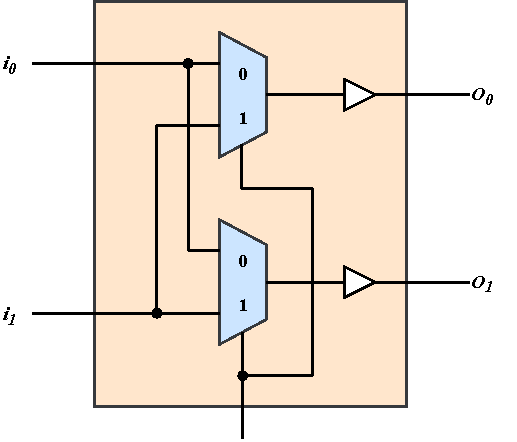
\includegraphics[width = 40mm]{figures/switch_block_detailed.pdf}
        \end{flushright}
    \end{wrapfigure}
    
    \vspace{1cm}
    
    {\normalsize
    \begin{tabular}{ r l }
    Examiner: & Prof. Dr. Elena Dubrova\\
    Supervisor: & Dr. Felipe Marranghello
    \end{tabular}}
\end{frame}

\begin{frame}{Today}
    \begin{itemize}[itemsep=0.25cm]
        \item \textbf{Motivation} - Why should you care?
        \item \textbf{Background} - What do I need to know?
        \item \textbf{Arbiter PUFs} - What are they?
        \item \textbf{Example} - How does it work?
        \item \textbf{Proof of Conflict} - What's the problem?
        \item \textbf{Solution} - How do we fix it?
        \item \textbf{Simulation} - What did we do?
        \item \textbf{Results} - What did we find?
        \item \textbf{Summary} - In short?
        \item \textbf{Conclusion} - And what?
    \end{itemize}
\end{frame}

\section{Motivation}

\begin{frame}{Motivation}
    \begin{center}
        \LARGE\textbf{50 billion IoT devices by 2020}
    \end{center}
\end{frame}

\begin{frame}{Motivation}
    \begin{itemize}[itemsep=0.5cm]
        \item \textbf{50 billion IoT devices by 2020:}
        \begin{itemize}
            \item DDoS attacks e.g. Dyn cyberattack 2016
        \end{itemize}
        \item \textbf{Intellectual property theft:} 
        \begin{itemize}
            \item Unique device identifiers
            \item Secure key storage (not battery backed SRAM or eFuses)
        \end{itemize}
        \item \textbf{Devices using PUFs:}
        \begin{itemize}
            \item Xilinx Zynq Ultrascale+ 
            \item Altera Stratix 10 FPGAs
        \end{itemize}
    \end{itemize}
\end{frame}

\begin{frame}{Motivation}
    \begin{figure}
        \centering
        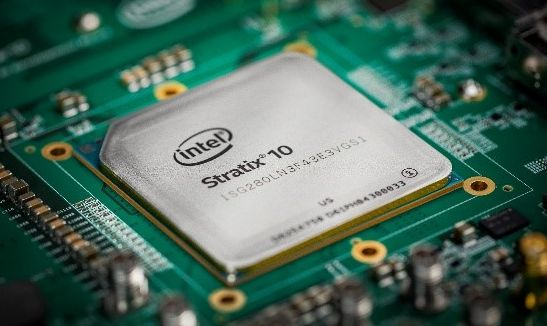
\includegraphics[width=0.7\textwidth]{figures/fpga.jpeg}
        \caption{Altera Stratix 10 FPGA}
    \end{figure}
\end{frame}

\section{Background}

\begin{frame}{Boolean Functions}
    \begin{table}[H]
        \centering
        \caption{There are ${2^2}^n$ different $n$-variable Boolean functions.}
        \def\arraystretch{1.5}
        \begin{tabular}{|c|l|}
        \hline
        No. of variables ($n$)  & Number of different functions ($f$)                                               \\ \hline
        1                       & 4 ($0, 1, x, \overline{x}$)	                                                    \\ \hline
        2                       & 16 ($0, 1, x_1, x_2, \overline{x_1}, \overline{x_2}, x_1 \xor x_2$, etc)          \\ \hline
        3                       & 256 ($0, 1, x_1, x_3, \overline{x_1}, \overline{x_2}, x_2 \xor x_3$, etc)         \\ \hline
        4                       & 65,536 ($0, 1, x_1, x_4, \overline{x_1}, \overline{x_2}, x_3 \xor x_4$, etc)      \\ \hline
        \vdots                  & \vdots                                                                            \\ \hline
        $n$                     & ${2^2}^n$ ($0, 1, x_1, x_n, \overline{x_1}, \overline{x_2}, x_3 \xor x_n$, etc)   \\ \hline
        \end{tabular}
    \end{table}
\end{frame}

\begin{frame}{Physical Unclonable Functions}
    \begin{itemize}[itemsep=0.5cm]
        \item \textbf{Digital fingerprint} for Integrated circuits
        \item \textbf{Manufacturing differences} give rise to a race condition
        \item \textbf{Mapping} between \textit{challenges} and \textit{responses}
        \item \textbf{Challenge Response Pair (CRP)} can be evaluated in the form of a \textbf{Boolean Function}
    \end{itemize}
\end{frame}

\section{Abiter PUFs} % yes or no?

\begin{frame}{Switch Block}
    \begin{figure}
        \centering
        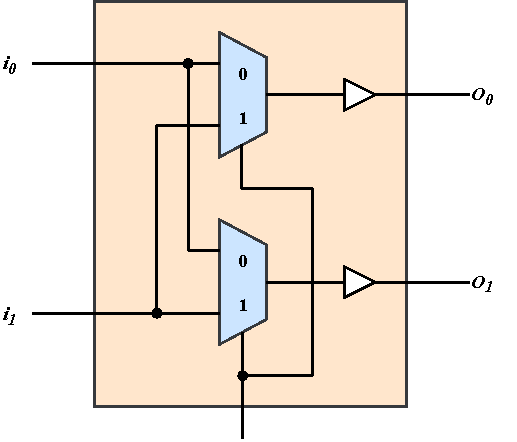
\includegraphics[width=0.6\textwidth]{figures/switch_block_detailed.pdf}
        \caption{Schematic of a switch block}
    \end{figure}
\end{frame}

\begin{frame}{Arbiter PUFs}
    \begin{figure}[ht]
        \centering
        \begin{subfigure}[b]{0.58\textwidth}
            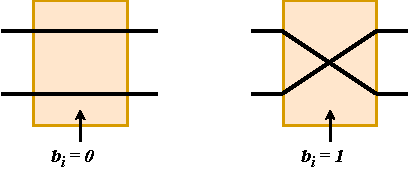
\includegraphics[width=\textwidth]{figures/switch_block_operations.pdf}
            \label{fig:switch_block_operations}
        \end{subfigure}
        \begin{subfigure}[b]{0.33\textwidth}
            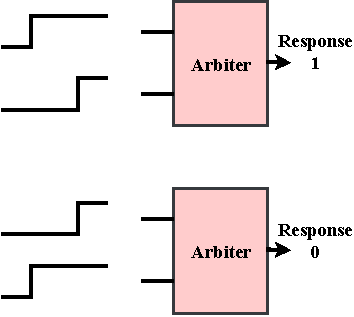
\includegraphics[width=\textwidth]{figures/arbiter_operation.pdf}
            \label{fig:arbiter_operations}
        \end{subfigure}
        \caption{Arbiter PUF operations}\label{fig:puf_operations}
    \end{figure}
\end{frame}

\begin{frame}{Arbiter PUFs}
    \begin{figure}
        \centering
        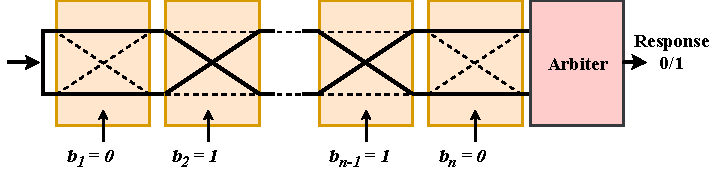
\includegraphics[width=\textwidth]{figures/multiple_switch_blocks.pdf}
        \caption{Multiple switch blocks in series form a PUF}
    \end{figure}
\end{frame}

\section{Example}

% \begin{frame}{Previous Studies}
% 	\begin{itemize}
% 		\item Machine Learning attacks
%         \item Stability
% 	\end{itemize}
% \end{frame}

\begin{frame}{Example}
    % \vspace*{-0.5cm}
    \begin{table}[H]
        \centering
        \begin{tabular}{cccc}
        $d_{11}$ = 1.1 ns & $d_{13}$ = 1.0 ns & $d_{21}$ = 1.2 ns & $d_{23}$ = 0.8 ns\\
        $d_{12}$ = 1.3 ns & $d_{14}$ = 1.5 ns & $d_{22}$ = 1.4 ns & $d_{24}$ = 0.9 ns\\
        \end{tabular}
    \end{table}
    % \vspace{-0.5cm}
    \begin{figure}
        \centering
        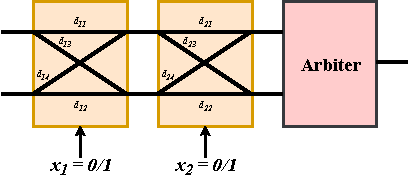
\includegraphics[width=\textwidth]{figures/2_switch_blocks_paths.pdf}
        \caption{Delay Paths}
    \end{figure}
\end{frame}

\begin{frame}{Example}
    \vspace*{-0.25cm}
    \begin{table}[H]
        \centering
        \begin{tabular}{cccc}
        $d_{11}$ = 1.1 ns & $d_{13}$ = 1.0 ns & $d_{21}$ = 1.2 ns & $d_{23}$ = 0.8 ns\\
        $d_{12}$ = 1.3 ns & $d_{14}$ = 1.5 ns & $d_{22}$ = 1.4 ns & $d_{24}$ = 0.9 ns\\
        \end{tabular}
    \end{table}
    \vspace{-0.5cm}
    
    \begin{figure}
        \centering
        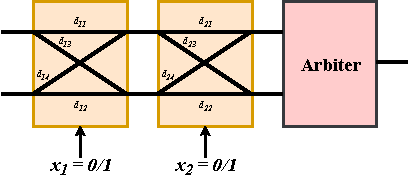
\includegraphics[width=0.6\textwidth]{figures/2_switch_blocks_paths.pdf}
    \end{figure}

    \begin{wrapfigure}{r}{0.2\textwidth}
        \begin{flushright}
        \vspace{-1cm}
        \begin{tabular}{ll|l}
\multicolumn{1}{c}{$x_1$} & \multicolumn{1}{c|}{$x_2$} & \multicolumn{1}{c}{$f$} \\ \hline
0                      & 0                      & 0                     \\
0                      & 1                      & 1                     \\
1                      & 0                      & 1                     \\
1                      & 1                      & 0                    
\end{tabular}
        \end{flushright}
    \end{wrapfigure}
    
    \vspace{-0.5cm}
    
    $(x_1,x_2) = (0,0) : d_{11}+d_{21} < d_{12}+d_{22} \to 0$
        
    $(x_1,x_2) = (0,1) : d_{12}+d_{24} > d_{11}+d_{23} \to 1$
        
    $(x_1,x_2) = (1,0) : d_{14}+d_{21} > d_{13}+d_{22} \to 1$
        
    $(x_1,x_2) = (1,1) : d_{13}+d_{24} > d_{14}+d_{23} \to 0$
    
    \vspace{0.5cm}
    
     The Boolean function induced by the PUF is $\mathbf{f(x_1, x_2) = x_1 \xor x_2}$, where "$\xor$" denotes XOR.
\end{frame}

\begin{frame}{Truth Table}
  \begin{table}[ht]
    \centering
    \caption{4 Boolean functions induced by an arbiter PUF with one switch block.}
    \def\arraystretch{1.2}
    $\begin{tabu}{c|c|c|c}
         \cline{2-3}
         & \multicolumn{2}{c|}{\text{Challenge}}                      &                                        \\ \cline{2-4}
                                  & x_1 = 0         & x_1 = 1         & \multicolumn{1}{||c|}{f(x_1)}          \\ \hline \tabucline[2pt]{-}
         \multicolumn{1}{|c|}{00} & d_{11} < d_{12} & d_{13} > d_{14} & \multicolumn{1}{||c|}{0}               \\ \hline
         \multicolumn{1}{|c|}{01} & d_{11} < d_{12} & d_{13} < d_{14} & \multicolumn{1}{||c|}{1}               \\ \hline
         \multicolumn{1}{|c|}{10} & d_{11} > d_{12} & d_{13} < d_{14} & \multicolumn{1}{||c|}{x_1}             \\ \hline
         \multicolumn{1}{|c|}{11} & d_{11} > d_{12} & d_{13} > d_{14} & \multicolumn{1}{||c|}{\overline{x_1}}  \\ \hline
    \end{tabu}$
\end{table}
\end{frame}

\begin{frame}{Truth Table}
  \begin{table}[ht]
    \centering
    \label{truth_table_2_bit}
  \def\arraystretch{1.2}
  \resizebox{\linewidth}{!}{  
    $\begin{tabu}{c|c|c|c|c|c}
        \cline{2-5}
        & \multicolumn{4}{c|}{\text{Challenge}}                        &                                                                                                                                                               \\ \cline{2-6}
                                   & x_2 x_1 = 0 0                     & x_2 x_1 = 0 1                     & x_2 x_1 = 1 0                     & x_2 x_1 = 1 1                     & \multicolumn{1}{||c|}{f(x_1, x_2)}                \\ \tabucline[2pt]{-}
        \multicolumn{1}{|c|}{0000} & d_{11} + d_{21} < d_{12} + d_{22} & d_{14} + d_{21} < d_{13} + d_{22} & d_{12} + d_{24} < d_{11} + d_{23} & d_{13} + d_{24} < d_{14} + d_{23} & \multicolumn{1}{||c|}{0}                          \\ \hline
        \multicolumn{1}{|c|}{0001} & d_{11} + d_{21} < d_{12} + d_{22} & d_{14} + d_{21} < d_{13} + d_{22} & d_{12} + d_{24} < d_{11} + d_{23} & d_{13} + d_{24} > d_{14} + d_{23} & \multicolumn{1}{||c|}{x_1 x_2}                    \\ \hline
        \multicolumn{1}{|c|}{0010} & d_{11} + d_{21} < d_{12} + d_{22} & d_{14} + d_{21} < d_{13} + d_{22} & d_{12} + d_{24} > d_{11} + d_{23} & d_{13} + d_{24} < d_{14} + d_{23} & \multicolumn{1}{||c|}{\overline{x_1} x_2}         \\ \hline
        \multicolumn{1}{|c|}{0011} & d_{11} + d_{21} < d_{12} + d_{22} & d_{14} + d_{21} < d_{13} + d_{22} & d_{12} + d_{24} > d_{11} + d_{23} & d_{13} + d_{24} > d_{14} + d_{23} & \multicolumn{1}{||c|}{x_2}                        \\ \hline
        \multicolumn{1}{|c|}{0100} & d_{11} + d_{21} < d_{12} + d_{22} & d_{14} + d_{21} > d_{13} + d_{22} & d_{12} + d_{24} < d_{11} + d_{23} & d_{13} + d_{24} < d_{14} + d_{23} & \multicolumn{1}{||c|}{x_1 \overline{x_2}}         \\ \hline
        \multicolumn{1}{|>{\columncolor[gray]{.8}}c|}{0101} & d_{11} + d_{21} < d_{12} + d_{22} & d_{14} + d_{21} > d_{13} + d_{22} & d_{12} + d_{24} < d_{11} + d_{23} & d_{13} + d_{24} > d_{14} + d_{23} & \multicolumn{1}{||>{\columncolor[gray]{.8}}c|}{x_1}                        \\ \hline
        \multicolumn{1}{|c|}{0110} & d_{11} + d_{21} < d_{12} + d_{22} & d_{14} + d_{21} > d_{13} + d_{22} & d_{12} + d_{24} > d_{11} + d_{23} & d_{13} + d_{24} < d_{14} + d_{23} & \multicolumn{1}{||c|}{x_1 \xor x_2}               \\ \hline
        \multicolumn{1}{|c|}{0111} & d_{11} + d_{21} < d_{12} + d_{22} & d_{14} + d_{21} > d_{13} + d_{22} & d_{12} + d_{24} > d_{11} + d_{23} & d_{13} + d_{24} > d_{14} + d_{23} & \multicolumn{1}{||c|}{x_1 + x_2}                  \\ \hline
        \multicolumn{1}{|c|}{1000} & d_{11} + d_{21} > d_{12} + d_{22} & d_{14} + d_{21} < d_{13} + d_{22} & d_{12} + d_{24} < d_{11} + d_{23} & d_{13} + d_{24} < d_{14} + d_{23} & \multicolumn{1}{||c|}{\overline{x_1 + x_2}}       \\ \hline
        \multicolumn{1}{|c|}{1001} & d_{11} + d_{21} > d_{12} + d_{22} & d_{14} + d_{21} < d_{13} + d_{22} & d_{12} + d_{24} < d_{11} + d_{23} & d_{13} + d_{24} > d_{14} + d_{23} & \multicolumn{1}{||c|}{\overline{x_1 \xor x_2}}    \\ \hline
        \multicolumn{1}{|>{\columncolor[gray]{.8}}c|}{1010} & d_{11} + d_{21} > d_{12} + d_{22} & d_{14} + d_{21} < d_{13} + d_{22} & d_{12} + d_{24} > d_{11} + d_{23} & d_{13} + d_{24} < d_{14} + d_{23} & \multicolumn{1}{||>{\columncolor[gray]{.8}}c|}{\overline{x_1}}             \\ \hline
        \multicolumn{1}{|c|}{1011} & d_{11} + d_{21} > d_{12} + d_{22} & d_{14} + d_{21} < d_{13} + d_{22} & d_{12} + d_{24} > d_{11} + d_{23} & d_{13} + d_{24} > d_{14} + d_{23} & \multicolumn{1}{||c|}{\overline{x_1} + x_2}       \\ \hline
        \multicolumn{1}{|c|}{1100} & d_{11} + d_{21} > d_{12} + d_{22} & d_{14} + d_{21} > d_{13} + d_{22} & d_{12} + d_{24} < d_{11} + d_{23} & d_{13} + d_{24} < d_{14} + d_{23} & \multicolumn{1}{||c|}{\overline{x_2}}             \\ \hline
        \multicolumn{1}{|c|}{1101} & d_{11} + d_{21} > d_{12} + d_{22} & d_{14} + d_{21} > d_{13} + d_{22} & d_{12} + d_{24} < d_{11} + d_{23} & d_{13} + d_{24} > d_{14} + d_{23} & \multicolumn{1}{||c|}{x_1 + \overline{x_2}}       \\ \hline
        \multicolumn{1}{|c|}{1110} & d_{11} + d_{21} > d_{12} + d_{22} & d_{14} + d_{21} > d_{13} + d_{22} & d_{12} + d_{24} > d_{11} + d_{23} & d_{13} + d_{24} < d_{14} + d_{23} & \multicolumn{1}{||c|}{\overline{x_1x_2}}          \\ \hline
        \multicolumn{1}{|c|}{1111} & d_{11} + d_{21} > d_{12} + d_{22} & d_{14} + d_{21} > d_{13} + d_{22} & d_{12} + d_{24} > d_{11} + d_{23} & d_{13} + d_{24} > d_{14} + d_{23} & \multicolumn{1}{||c|}{1}                          \\ \hline
    \end{tabu}$ 
    }
\end{table}
\end{frame}


\begin{frame}{proof of conflict}
    \begin{center}
        For $\mathbf{f(x_1, x_2) = x_1}$
        
        \vspace{0,5cm}
    
        $d_{11} + d_{21} < d_{12} + d_{22}$
        
        $d_{14} + d_{21} > d_{13} + d_{22}$
        
        $d_{12} + d_{24} < d_{11} + d_{23}$
        
        $d_{13} + d_{24} > d_{14} + d_{23}$
        
        \vspace{0.5cm}

        $-\Delta_{11-12} < \Delta_{13-14} < -\Delta_{11-12}$
        
        \vspace{0.5cm}
        
        Hence, $\mathbf{f(x_1, x_2) = x_1}$ can NOT be induced by a single arbiter PUF!
    \end{center}
\end{frame}

\section{Solution}

\begin{frame}{XORed PUFs}
    \begin{figure}
        \centering
        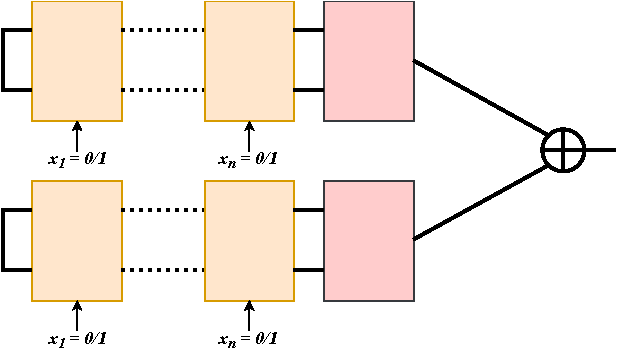
\includegraphics[width=0.7\textwidth]{figures/puf_2_xor.pdf}
        \caption{Setup for two XORed arbiter PUFs}
    \end{figure}
\end{frame}

\begin{frame}{Example}
    Two functions that can be induced by a single arbiter PUF:

        \[\mathbf{f(x_1, x_2) = x_1 \xor x_2}\]
    
        \[\mathbf{f(x_1, x_2) = x_2}\]
        
        \vspace{0.5cm}
        
        \[(x_1 \xor x_2) \xor x_2 = x_1 \xor x_2 \xor x_1 = \mathbf{x_1}\]
        
        \vspace{1cm}
        
        \begin{center}
            \large\textbf{``Et Voilà!"}
        \end{center}
\end{frame}


% remove deltas no need - no need for working
% how can we solve this problem?
% introduce xor pufs
% how is the simulation done?
% explain the process of the simulation
% conclusion we show the distribution is not uniform 
% potential weekness, xoring can improve it.


\section{Simulation}

\begin{frame}{Simulation}
    
    \begin{itemize}[itemsep=0.5cm]
        \item 1. Select \textbf{n} and \textbf{number of trials}
        \item 2. For each trial:
        \begin{itemize}[itemsep=0.25cm]
            \item • Assign random values to the delays (Gaussian Distribution)
            \item • Evaluate the resulting truth table
        \end{itemize}
    \end{itemize}
\end{frame}

\begin{frame}{Goal}
    \begin{center}
        \LARGE\textbf{We want uniform distribution!}
    \end{center}
\end{frame}

\section{Results}

% ----------
% SINGLE PUF
% ----------

\begin{frame}{Results}
    \begin{figure}
        \centering
        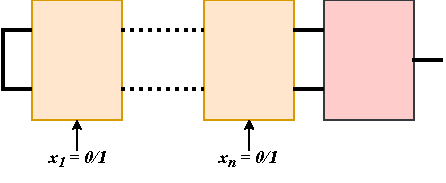
\includegraphics[width=0.7\textwidth]{figures/puf_1.pdf}
        \caption{Single Arbiter PUF}
    \end{figure}
\end{frame}

\begin{frame}{Single Arbiter PUF}
    \begin{figure}
        \centering
        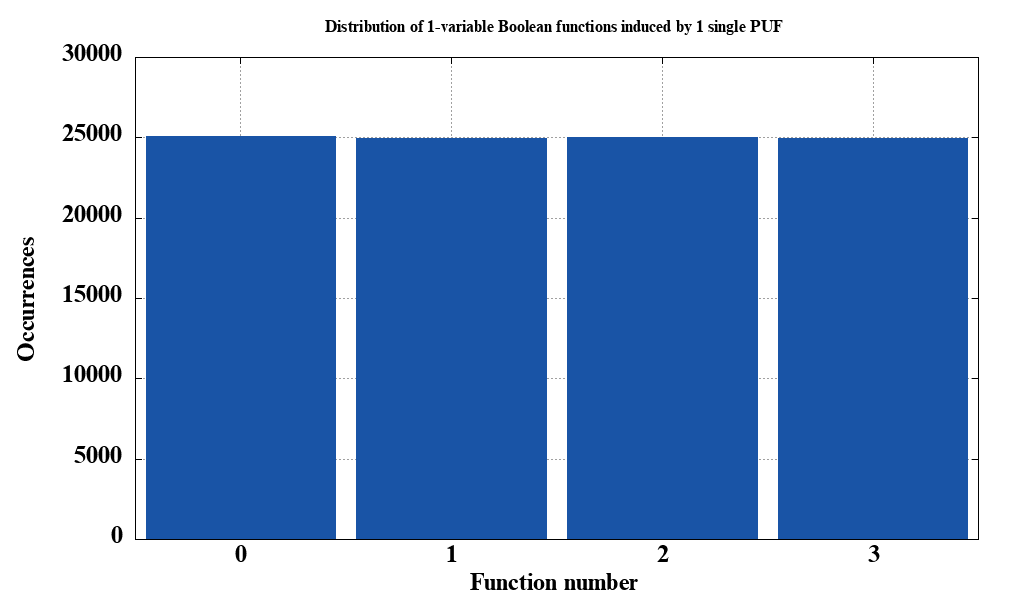
\includegraphics[width=\textwidth]{figures/dist/distribution_of_1-variable_boolean_functions_induced_by_1_single_puf.png}
        \caption{All functions are equally probable.}
    \end{figure}
\end{frame}

\begin{frame}{Single Arbiter PUF}
    \begin{figure}
        \centering
        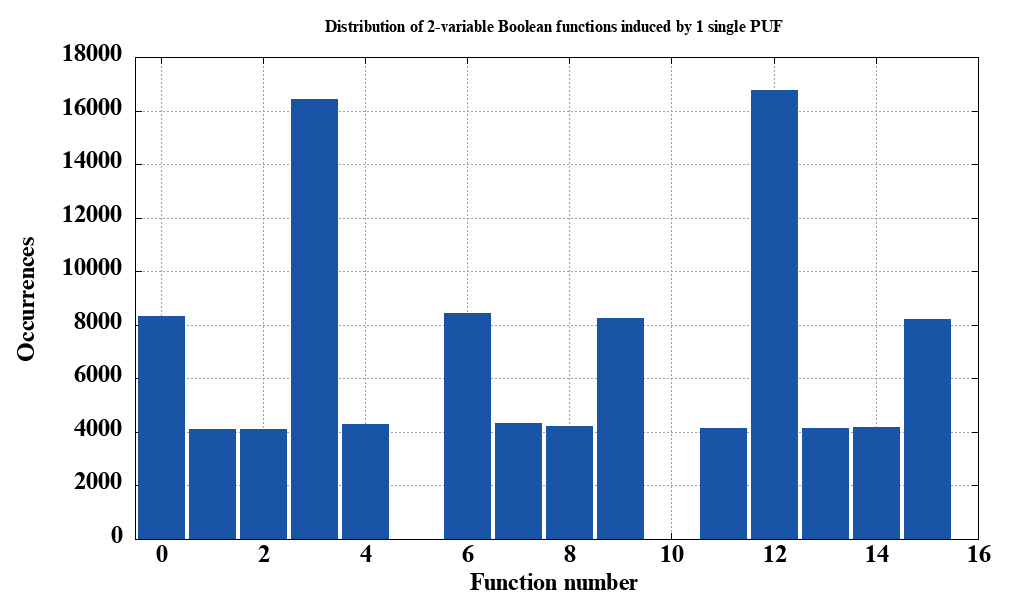
\includegraphics[width=\textwidth]{figures/dist/distribution_of_2-variable_boolean_functions_induced_by_1_single_puf.png}
        \caption{$x_1$ and $\overline{x_1}$ are not induced (100,000 trials).}
    \end{figure}
\end{frame}

\begin{frame}{Single Arbiter PUF}
    \begin{figure}
        \centering
        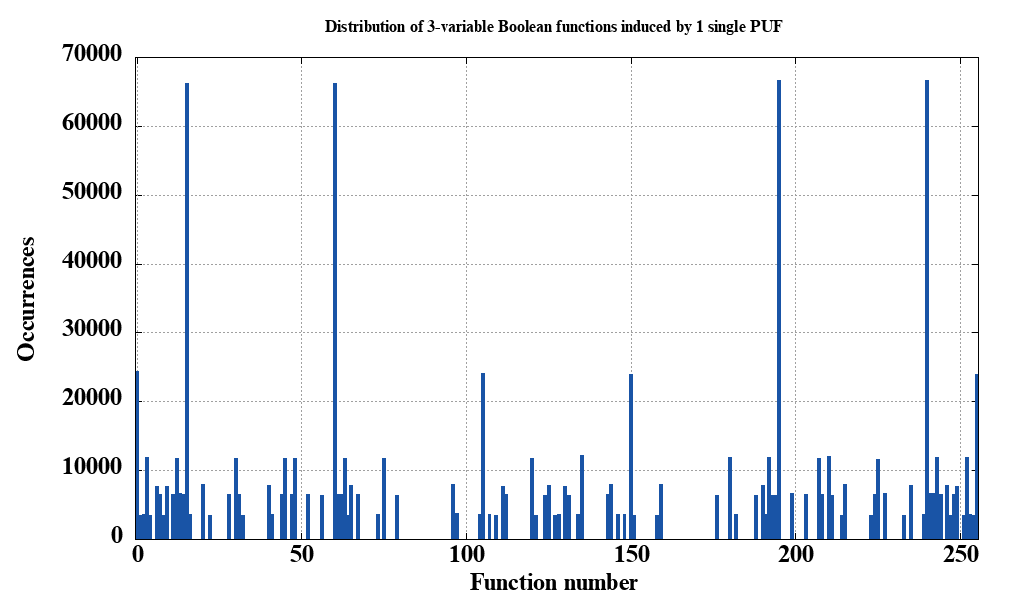
\includegraphics[width=\textwidth]{figures/dist/distribution_of_3-variable_boolean_functions_induced_by_1_single_puf.png}
        \caption{152 functions are not induced (1 million trials).}
    \end{figure}
\end{frame}

\begin{frame}{Single Arbiter PUF}
    \begin{figure}
        \centering
        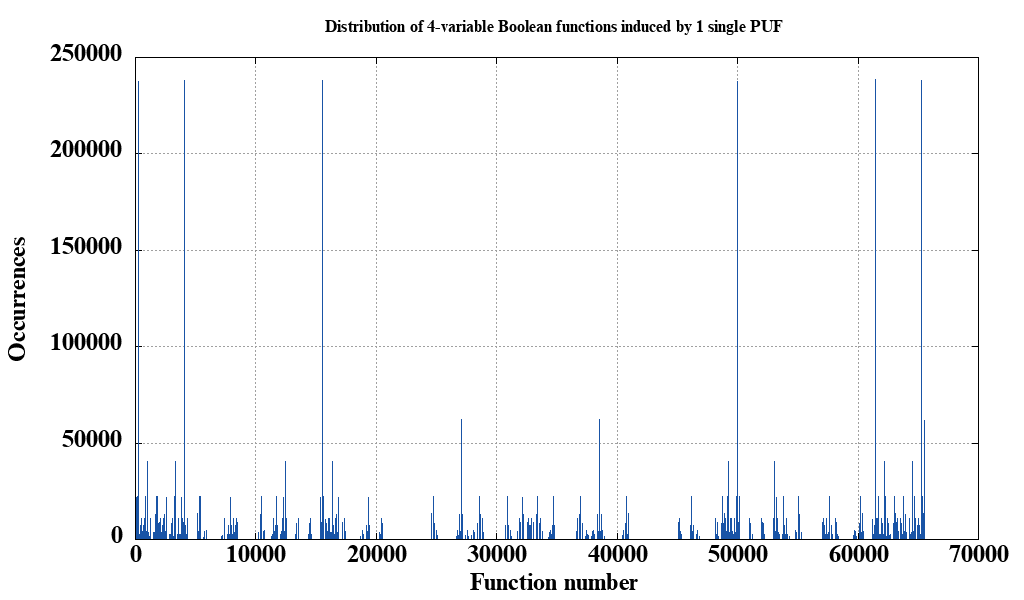
\includegraphics[width=\textwidth]{figures/dist/distribution_of_4-variable_boolean_functions_induced_by_1_single_puf.png}
        \caption{63,654 functions are not induced (10 million trials).}
    \end{figure}
\end{frame}

\section{Coverage}

\begin{frame}{Single Arbiter PUF}
    \begin{figure}
        \centering
        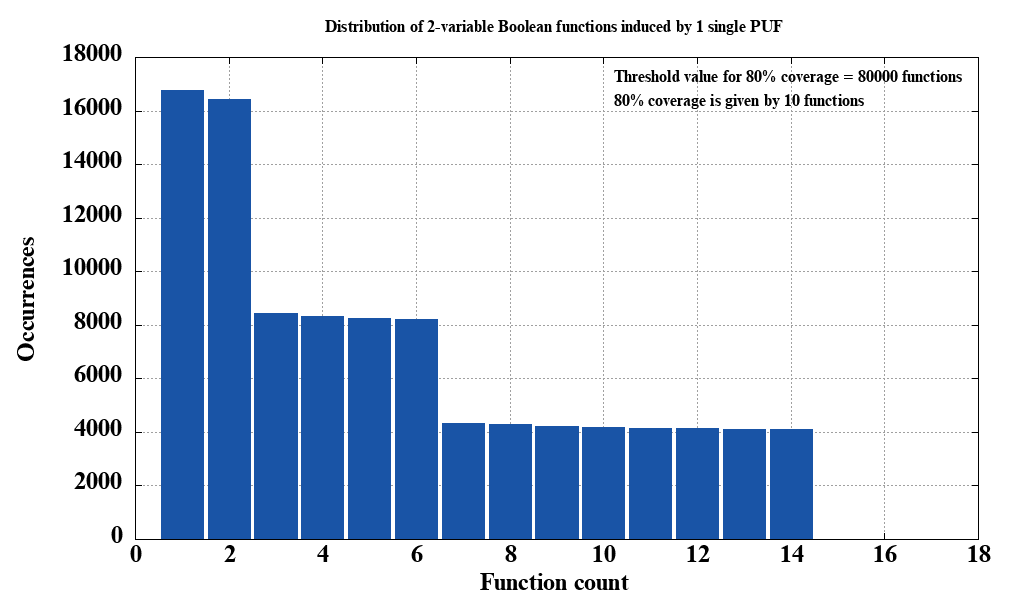
\includegraphics[width=\textwidth]{figures/sorted/distribution_of_2-variable_boolean_functions_induced_by_1_single_puf.png}
    \end{figure}
\end{frame}

\begin{frame}{Single Arbiter PUF}
    \begin{figure}
        \centering
        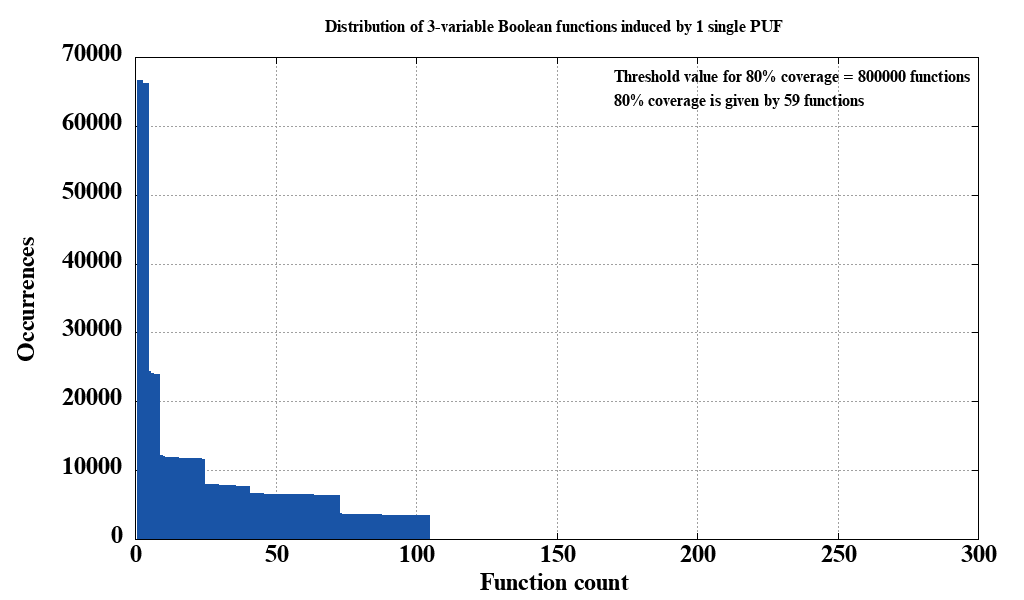
\includegraphics[width=\textwidth]{figures/sorted/distribution_of_3-variable_boolean_functions_induced_by_1_single_puf.png}
    \end{figure}
\end{frame}

\begin{frame}{Single Arbiter PUF}
    \begin{figure}
        \centering
        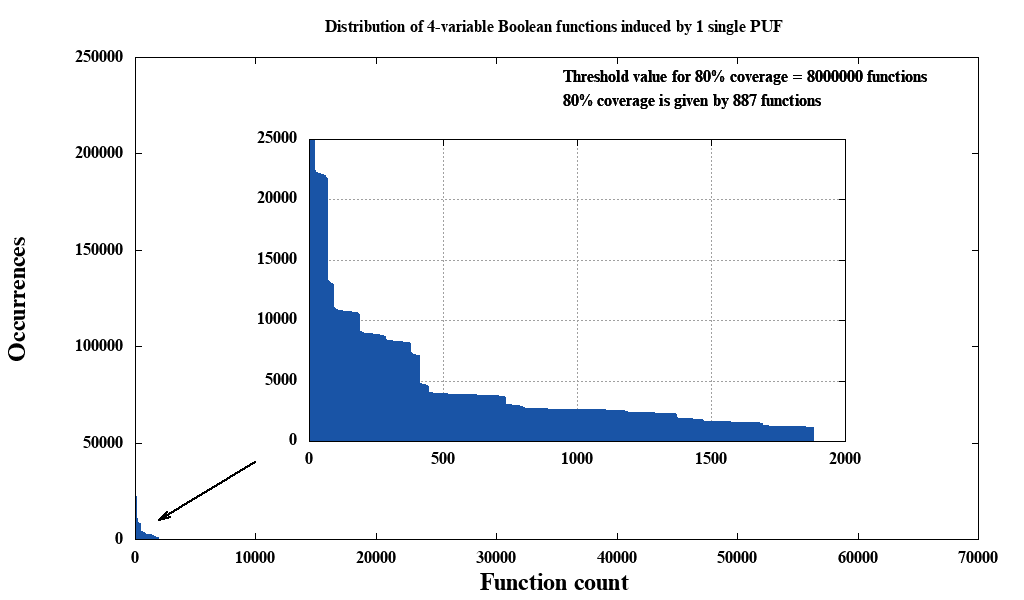
\includegraphics[width=\textwidth]{figures/zoom/distribution_of_4-variable_boolean_functions_induced_by_1_single_puf_zoom.png}
    \end{figure}
\end{frame}

% --------------
% TWO XORed PUFs
% --------------

\begin{frame}{Results}
    \begin{figure}
        \centering
        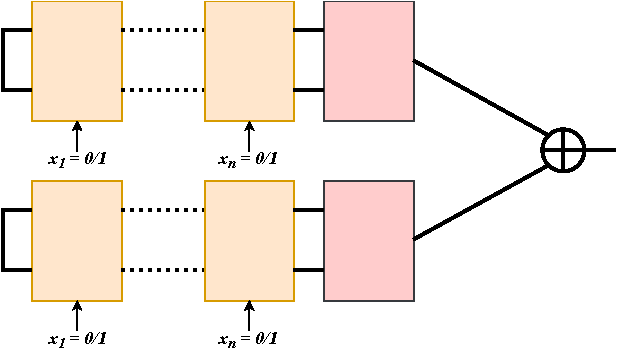
\includegraphics[width=0.7\textwidth]{figures/puf_2_xor.pdf}
        \caption{Two XORed PUFs}
    \end{figure}
\end{frame}

\begin{frame}{Two XORed PUFs}
    \begin{figure}
        \centering
        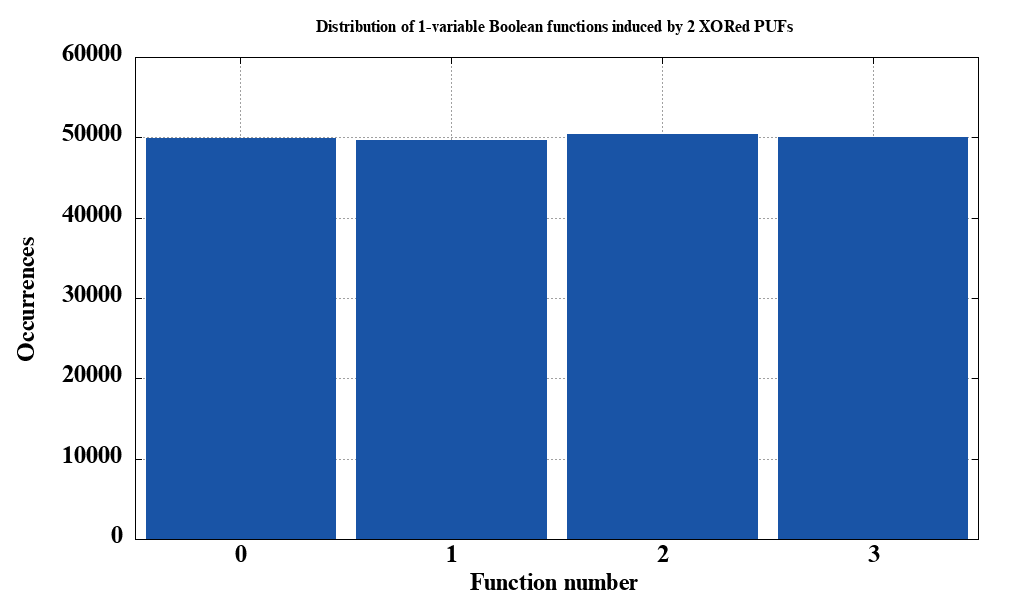
\includegraphics[width=\textwidth]{figures/dist/distribution_of_1-variable_boolean_functions_induced_by_2_xored_pufs.png}
        \caption{All functions are equally probable.}
    \end{figure}
\end{frame}

\begin{frame}{Two XORed PUFs}
    \begin{figure}
        \centering
        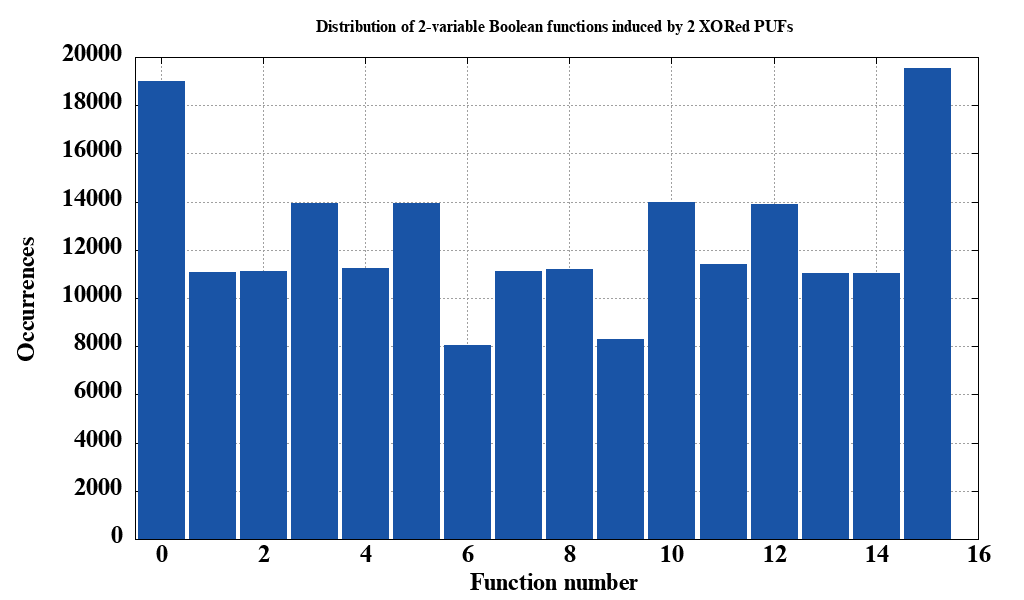
\includegraphics[width=\textwidth]{figures/dist/distribution_of_2-variable_boolean_functions_induced_by_2_xored_pufs.png}
        \caption{All functions are induced (100,000 trials).}
    \end{figure}
\end{frame}

\begin{frame}{Two XORed PUFs}
    \begin{figure}
        \centering
        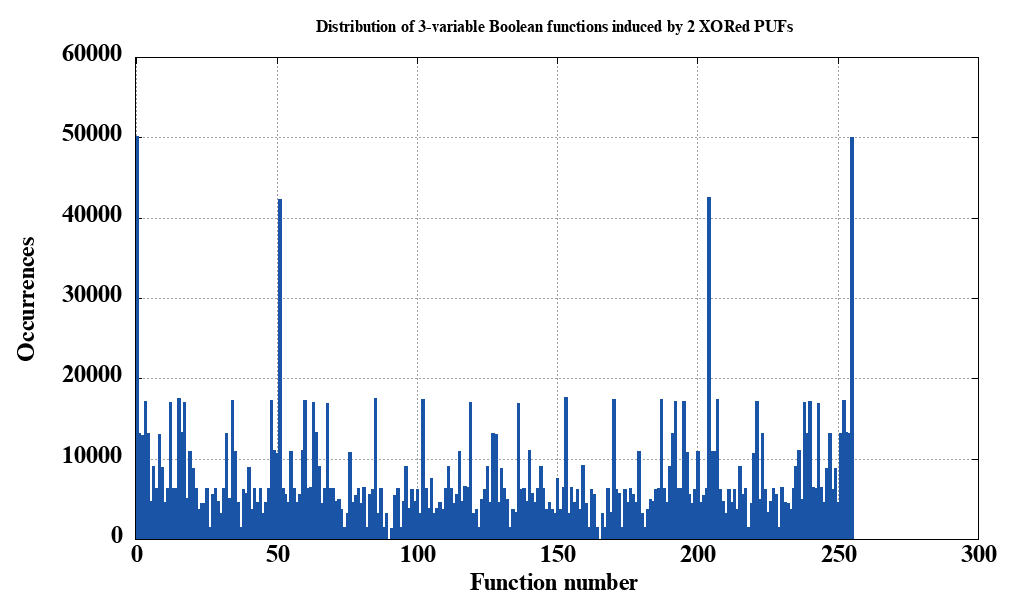
\includegraphics[width=\textwidth]{figures/dist/distribution_of_3-variable_boolean_functions_induced_by_2_xored_pufs.png}
        \caption{All functions excl. $x_1 \xor x_2$ and $\overline{x_1 \xor x_2}$ are induced (1 million trials).}
    \end{figure}
\end{frame}

\begin{frame}{Two XORed PUFs}
    \begin{figure}
        \centering
        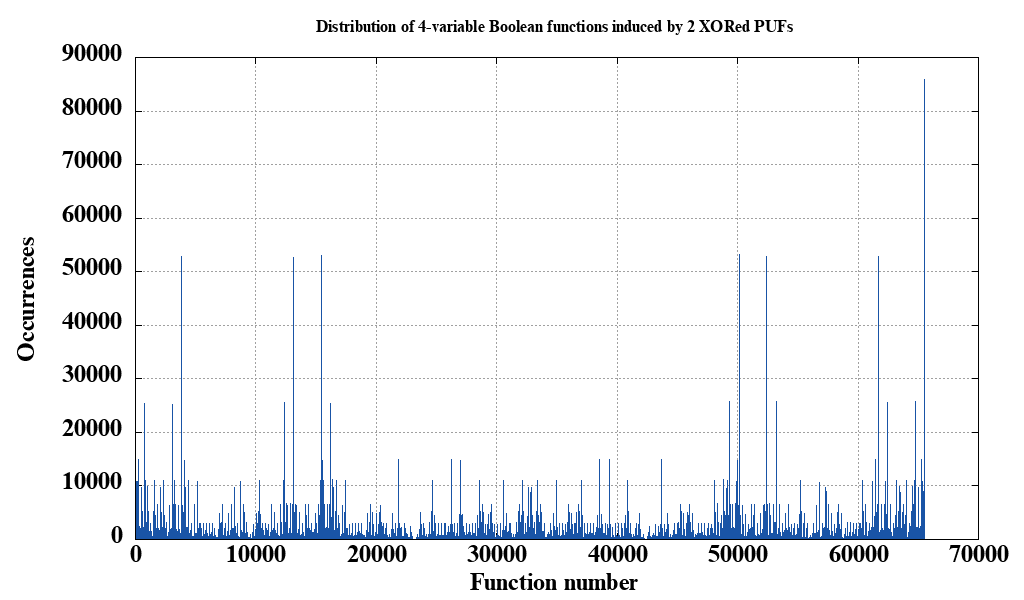
\includegraphics[width=\textwidth]{figures/dist/distribution_of_4-variable_boolean_functions_induced_by_2_xored_pufs.png}
        \caption{11,226 functions are not induced (100 million trials).}
    \end{figure}
\end{frame}

\section{Coverage}

\begin{frame}{Two XORed PUFs}
    \begin{figure}
        \centering
        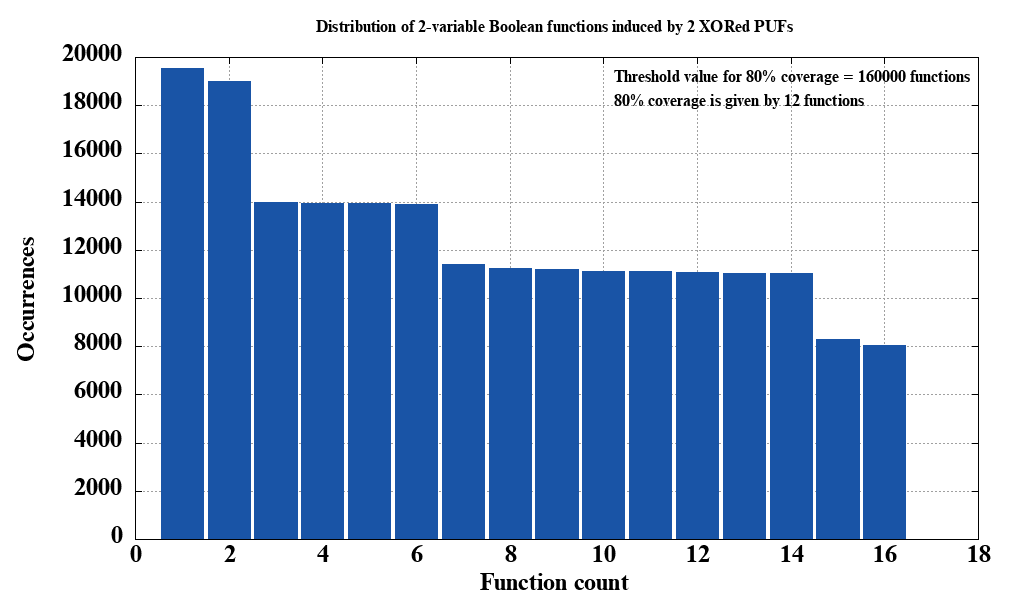
\includegraphics[width=\textwidth]{figures/sorted/distribution_of_2-variable_boolean_functions_induced_by_2_xored_pufs.png}
    \end{figure}
\end{frame}

\begin{frame}{Two XORed PUFs}
    \begin{figure}
        \centering
        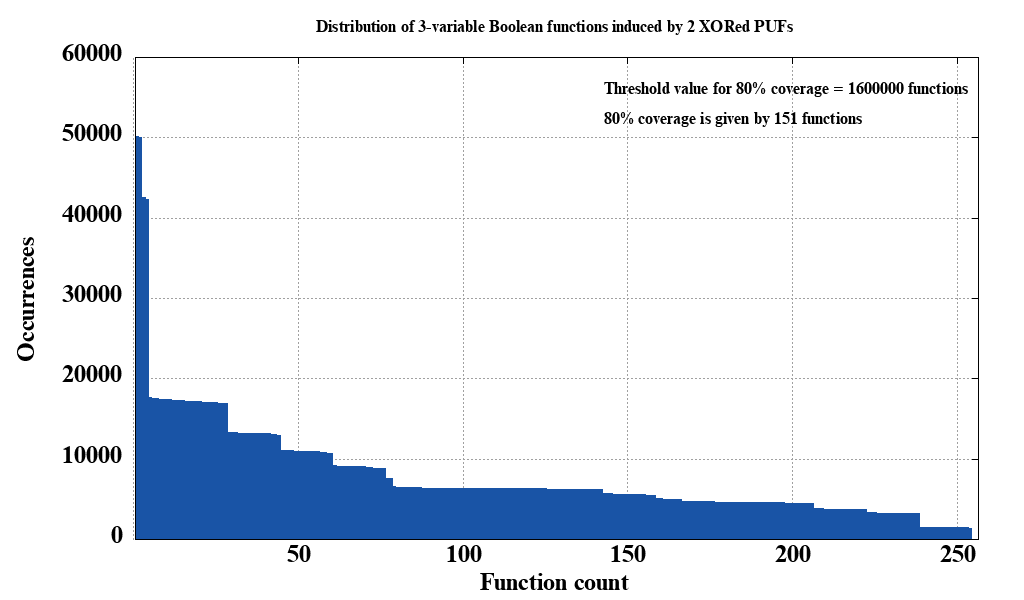
\includegraphics[width=\textwidth]{figures/sorted/distribution_of_3-variable_boolean_functions_induced_by_2_xored_pufs.png}
    \end{figure}
\end{frame}

\begin{frame}{Two XORed PUFs}
    \begin{figure}
        \centering
        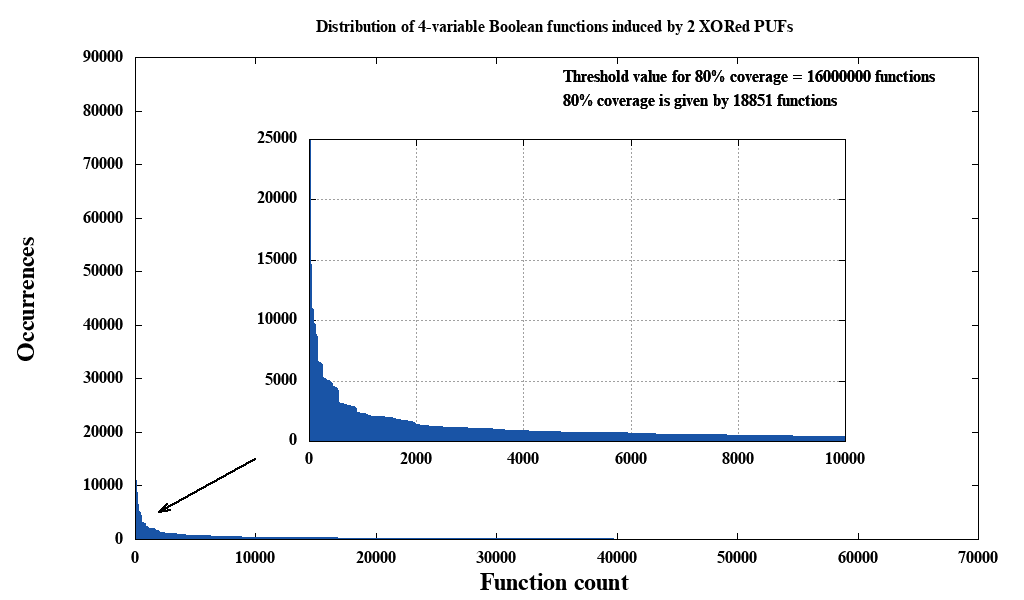
\includegraphics[width=\textwidth]{figures/zoom/distribution_of_4-variable_boolean_functions_induced_by_2_xored_pufs_zoom.png}
    \end{figure}
\end{frame}

% ----------------
% THREE XORed PUFs 
% ----------------

\begin{frame}{Results}
    \begin{figure}
        \centering
        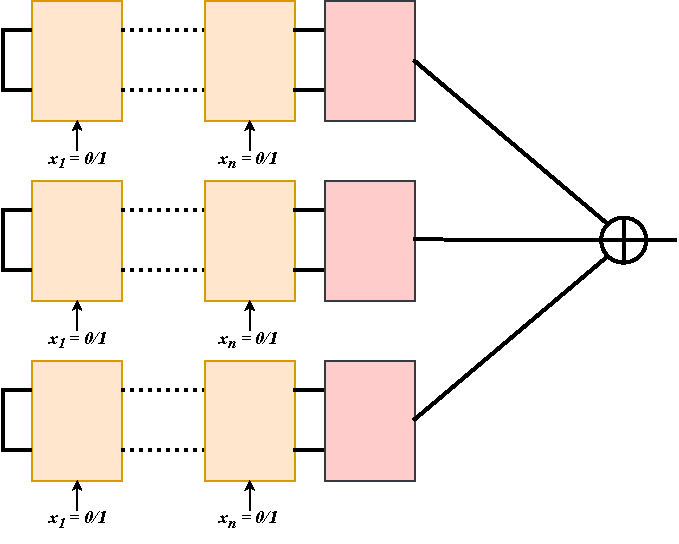
\includegraphics[width=0.7\textwidth]{figures/puf_3_xor.pdf}
        \caption{Three XORed PUFs}
    \end{figure}
\end{frame}

\begin{frame}{Three XORed PUFs}
    \begin{figure}
        \centering
        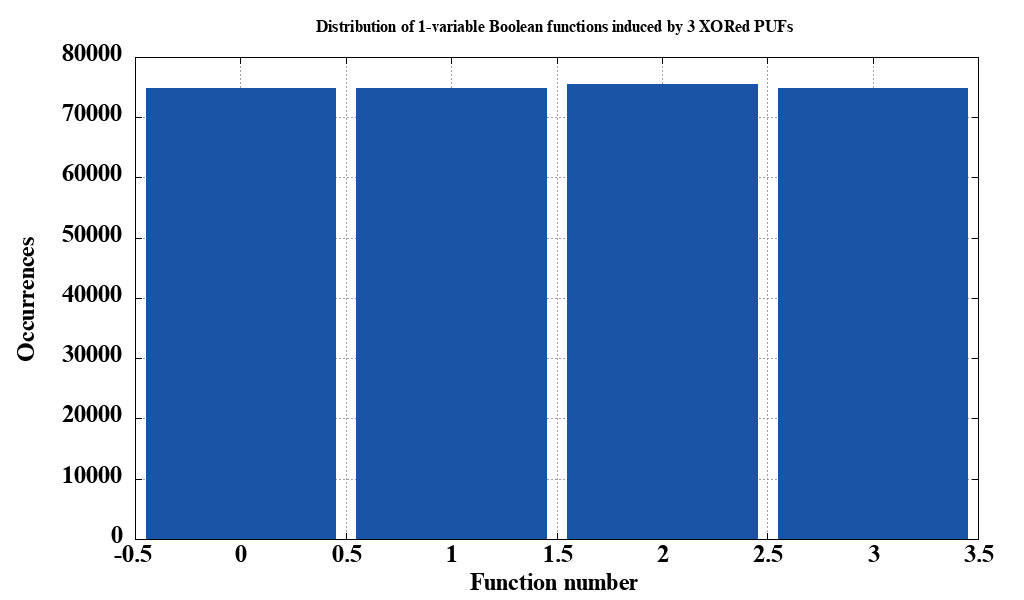
\includegraphics[width=\textwidth]{figures/dist/distribution_of_1-variable_boolean_functions_induced_by_3_xored_pufs.png}
        \caption{All functions are equally probable}
    \end{figure}
\end{frame}

\begin{frame}{Three XORed PUFs}
    \begin{figure}
        \centering
        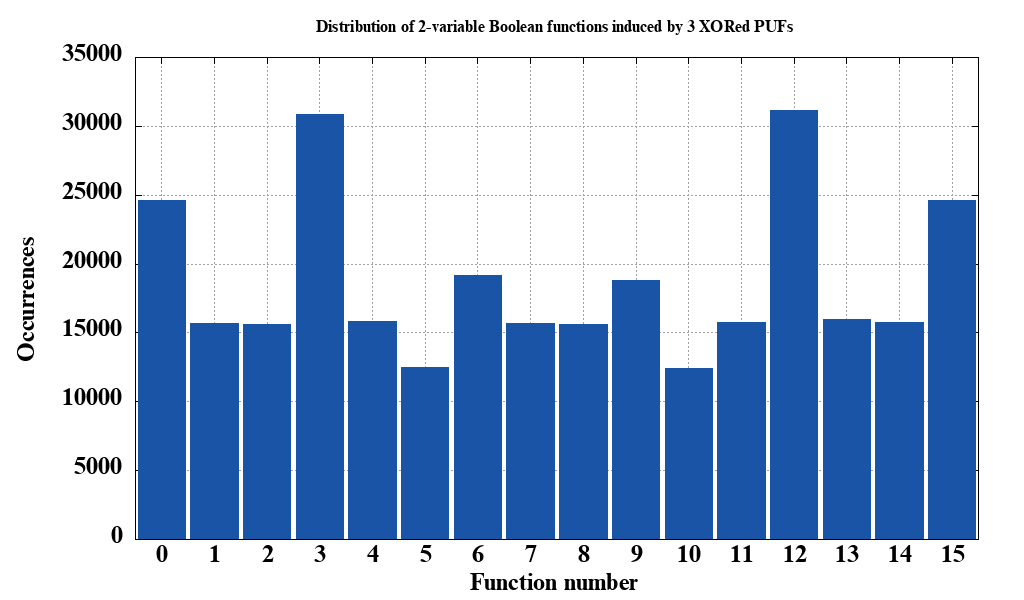
\includegraphics[width=\textwidth]{figures/dist/distribution_of_2-variable_boolean_functions_induced_by_3_xored_pufs.png}
        \caption{All functions are induced (100,000 trials).}
    \end{figure}
\end{frame}

\begin{frame}{Three XORed PUFs}
    \begin{figure}
        \centering
        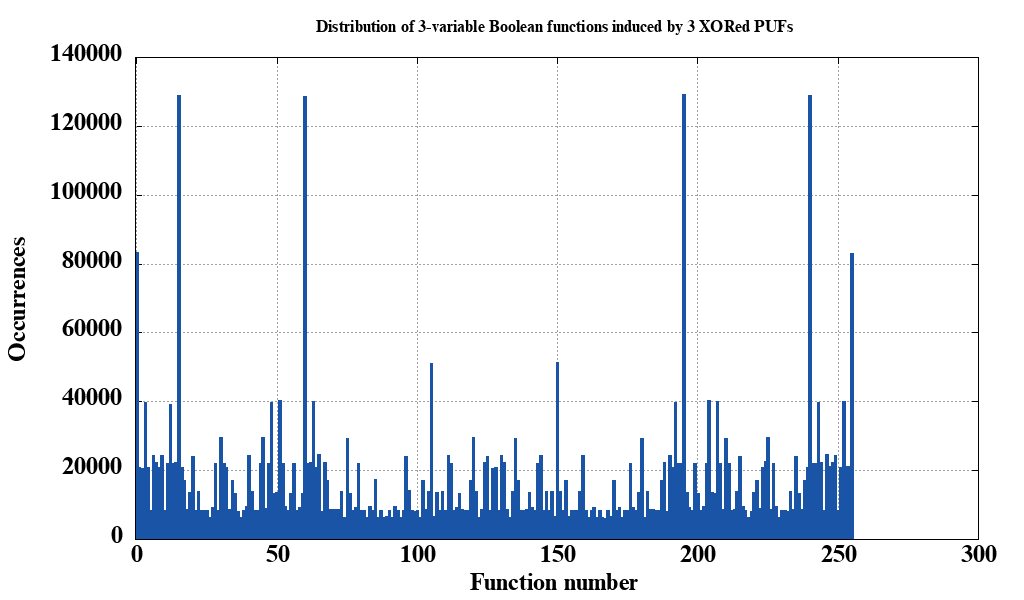
\includegraphics[width=\textwidth]{figures/dist/distribution_of_3-variable_boolean_functions_induced_by_3_xored_pufs.png}
        \caption{All functions are induced (1.5 million trials).}
    \end{figure}
\end{frame}

\begin{frame}{Three XORed PUFs}
    \begin{figure}
        \centering
        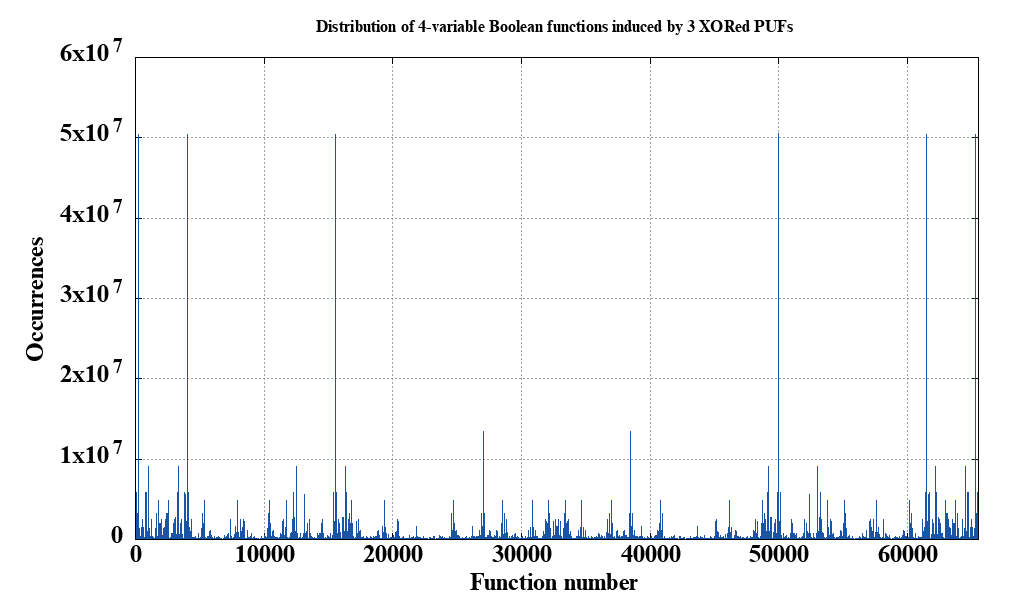
\includegraphics[width=\textwidth]{figures/dist/distribution_of_4-variable_boolean_functions_induced_by_3_xored_pufs.png}
        \caption{All functions excl. $x_1 \xor x_3$ and $\overline{x_1 \xor x_3}$ are induced (2 billion trials).}
    \end{figure}
\end{frame}

\section{Coverage}

\begin{frame}{Three XORed PUFs}
    \begin{figure}
        \centering
        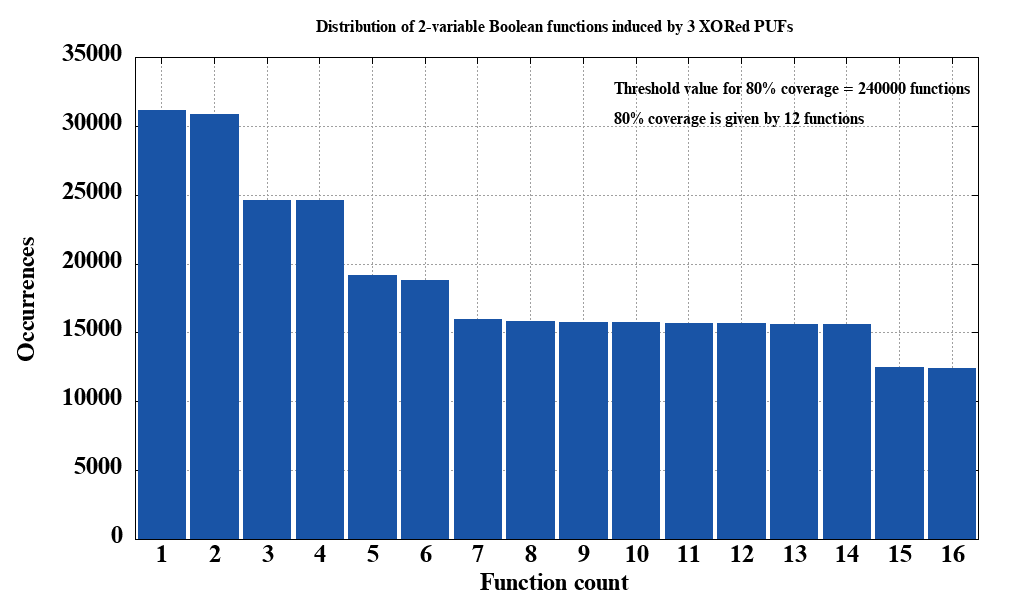
\includegraphics[width=\textwidth]{figures/sorted/distribution_of_2-variable_boolean_functions_induced_by_3_xored_pufs.png}
    \end{figure}
\end{frame}

\begin{frame}{Three XORed PUFs}
    \begin{figure}
        \centering
        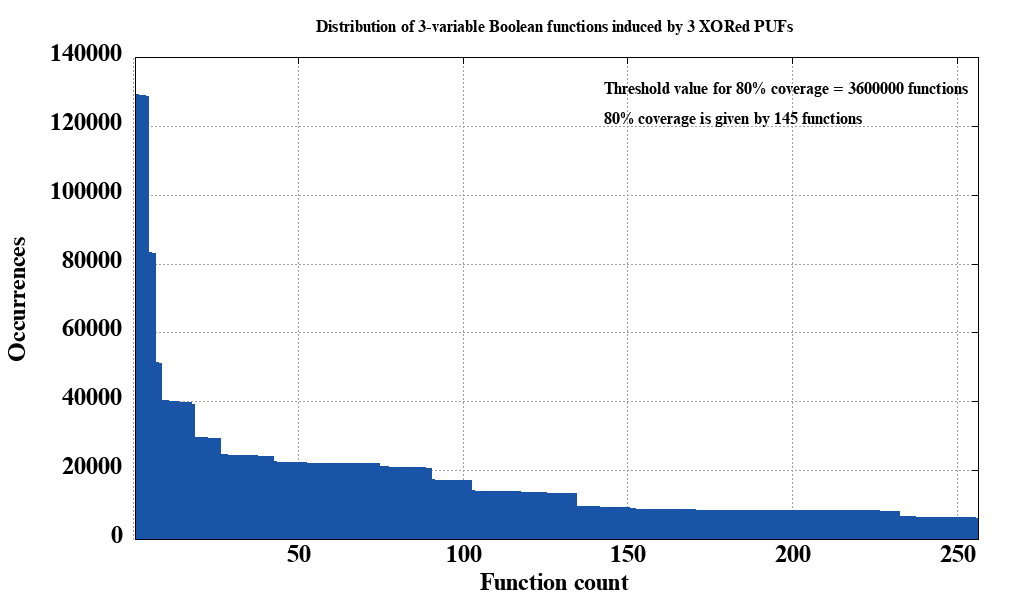
\includegraphics[width=\textwidth]{figures/sorted/distribution_of_3-variable_boolean_functions_induced_by_3_xored_pufs.png}
    \end{figure}
\end{frame}

\begin{frame}{Three XORed PUFs}
    \begin{figure}
        \centering
        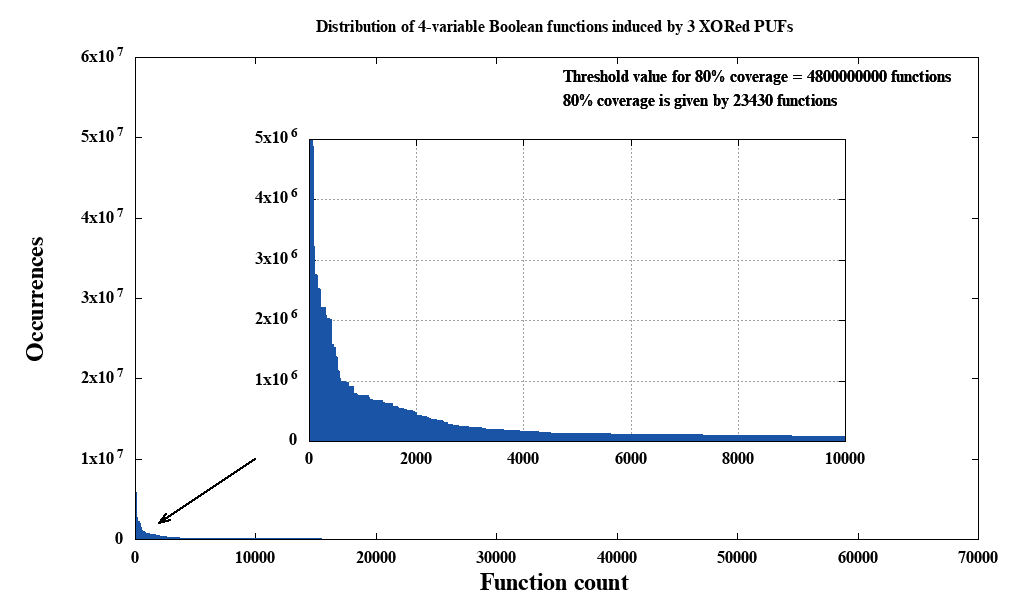
\includegraphics[width=\textwidth]{figures/zoom/distribution_of_4-variable_boolean_functions_induced_by_3_xored_pufs_zoom.png}
    \end{figure}
\end{frame}

\section{Summary}

\begin{frame}{Summary}
    \begin{figure}
        \centering
        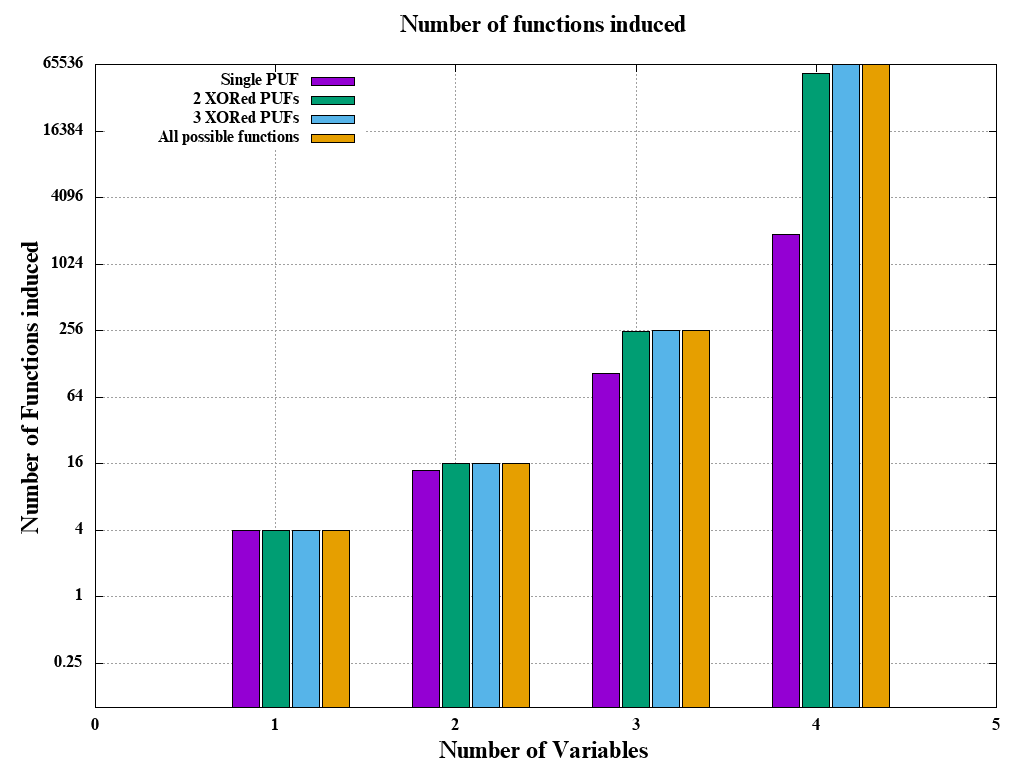
\includegraphics[width=0.9\textwidth]{figures/hist.png}
    \end{figure}
\end{frame}

\begin{frame}{Overview}
    \begin{table}[H]
    \caption{Number of Impossible Functions}
    \label{function_overview}    
    \def\arraystretch{1.45}
        \begin{subtable}{0.40\textwidth}
            \centering
            \begin{tabular}{|c|c|c|}
            \hline
            $n$     & $N$       & $I$                       \\ \Xhline{5\arrayrulewidth}
            1       & 4         & 0                         \\ \hline
            2       & 16        & 2                         \\ \hline
            3       & 256       & 152                       \\ \hline
            4       & 65,536    & 63,654                    \\ \hline
            \vdots  & \vdots    & \vdots                    \\ \hline
            $n$     & ${2^2}^n$ & $\geq	{2^2}^{n-1} - 2$    \\ \hline
            \end{tabular}
        \caption{One single PUF}
        \end{subtable}
        ~ 
        \begin{subtable}{0.28\textwidth}
            \centering
            \begin{tabular}{|c|c|}
            \hline
            $N$       & $I$       \\ \Xhline{5\arrayrulewidth}
            4         & 0         \\ \hline
            16        & 0         \\ \hline
            256       & 2         \\ \hline
            65,536    & 11,226    \\ \hline
            \vdots    & \vdots    \\ \hline
            ${2^2}^n$ & ???       \\ \hline
            \end{tabular}
        \caption{2 XORed PUFs}
        \end{subtable}
        ~
        \begin{subtable}{0.23\textwidth}
            \centering
            \begin{tabular}{|c|c|}
            \hline
            $N$       & $I$       \\ \Xhline{5\arrayrulewidth}
            4         & 0         \\ \hline
            16        & 0         \\ \hline
            256       & 0         \\ \hline
            65,536    & 2         \\ \hline
            \vdots    & \vdots    \\ \hline
            ${2^2}^n$ & ???       \\ \hline
            \end{tabular}
            \caption{3 XORed PUFs}
        \end{subtable}
    \end{table}
\end{frame}

\begin{frame}{Impossible Functions}
    \begin{table}[H]
        \centering
        \begin{tabular}{r l}
             $f(x_1,x_2) =  \begin{cases} 
                                    \overline{x_1}\\ 
                                    x_1
                                \end{cases}$ &  for $n=2$ using 1 single PUF \\
                                &\\
             $f(x_1,x_2,x_3) =  \begin{cases} 
                                    \overline{x_1 \xor x_2}\\ 
                                    x_1 \xor x_2
                                \end{cases}$ & for $n = 3$ using 2 XORed PUFs \\
                                &\\
             $f(x_1,x_2,x_3,x_4) =  \begin{cases} 
                                    \overline{x_1 \xor x_3}\\ 
                                    x_1 \xor x_3
                                \end{cases}$ & for $n = 4$ using 3 XORed PUFs
                                
        \end{tabular}
    \end{table}  
\end{frame}

\begin{frame}{Hypothesis}
    \begin{center}
        \LARGE\textbf{$\mathbf{n}$ XORed arbiter PUFs can induce all $\mathbf{{2^2}^n}$\\$\mathbf{n}$-variable Boolean functions.}
    \end{center}
\end{frame}

\begin{frame}{Hypothesis}
    \begin{figure}
        \centering
        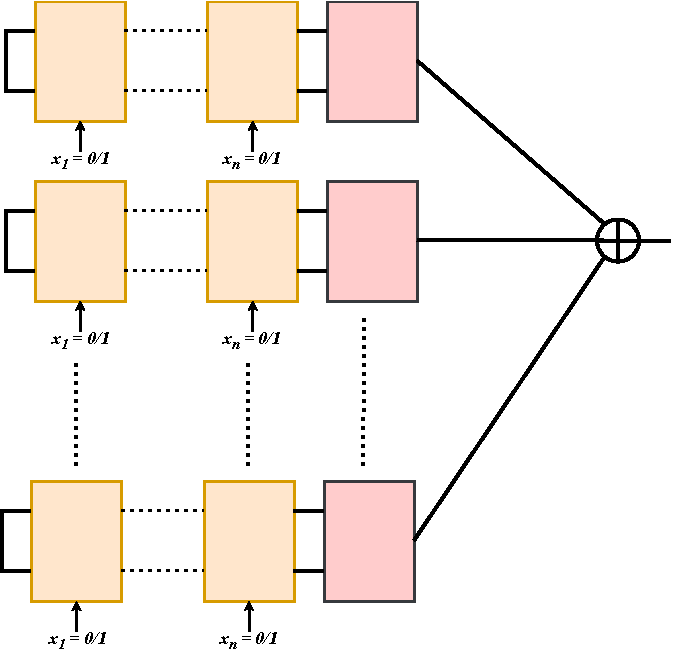
\includegraphics[width=0.6\textwidth]{figures/puf_n_xor.pdf}
        \caption{$n$ XORed PUFs can induce all possible $n$-variable functions.}
    \end{figure}
\end{frame}

\section{Conclusion}

\begin{frame}{Future Work}
    \begin{figure}
        \centering
        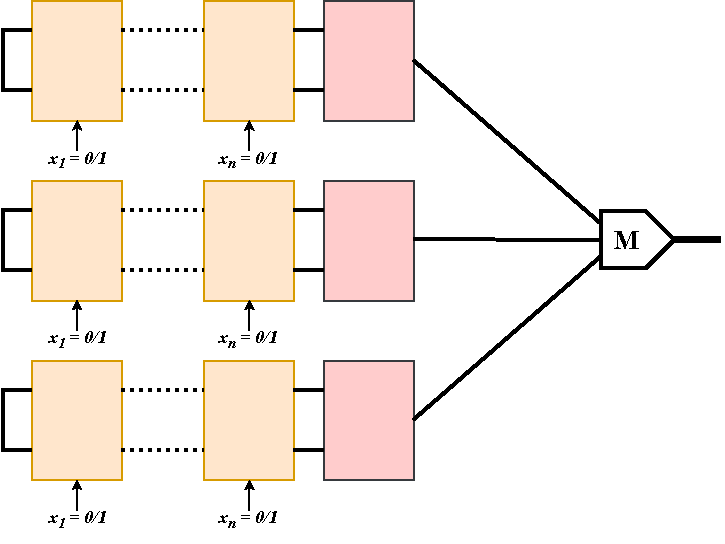
\includegraphics[width=0.6\textwidth]{figures/puf_3_maj.pdf}
        \caption{Three arbiter PUFs MAJed}
    \end{figure}
\end{frame}

\begin{frame}{Conclusion}
    \begin{itemize}[itemsep=1cm]
        \item Functions induced by arbiter PUFs are \textbf{not uniformly} distributed
        \item Potential \textbf{weakness} - could be used for targeted attacks
        \item \textbf{XORing} PUFs can improve the distribution
    \end{itemize}
\end{frame}

\begin{frame}{Acknowledgements}
    \begin{itemize}
        \item Latex Beamer:
    \end{itemize}
    \begin{center}\url{github.com/matze/mtheme}\end{center}
    \begin{itemize}
        \item Graphics:
    \end{itemize}    \begin{center}\url{draw.io}\end{center}
\end{frame}

\plain{}{Questions?}

\plain{}{Prof. Dr. Elena Dubrova\\Dr. Felipe Marranghello}

\end{document}